\chapter{The International Market Survey - Results}
\renewcommand{\arraystretch}{1.5}
This chapter is intended to present the results from the International Survey to the reader, with the questions and responses being presented and discussed here. In total, 193 different \glspl{hei} were contacted and 39 respondents submitted answers. This yields a response rate of over 20\%. 
\section{Respondents}
Replies from different countries are represented in Table~\ref{contactedcountries}, and geographically in Figure~\ref{fig:worldmap}. The color code used in this figure represents which countries that had \glspl{hei} contacted, where red indicates no reply from any \gls{hei} in that country, and green indicating one or more replies from a \gls{hei} in that country. The "Other" category that contains four possible answers, were respondents who failed to denote what institution they were representing, and no indication of who they were representing were given whatsoever. After the initial sendout, the chosen \glspl{hei} contacted were adjusted in order to obtain more data from the survey. This was done by contacting more \glspl{hei} from countries with a good response rate. Countries with English as a first language are also more represented, and as such there may exist a correlation between this and the response rate from these countries. In general more European countries replied to the survey, and apart from any possible language barriers, the websites of \glspl{hei} from western countries were generally more open and informative, making it easier to find the correct person to contact. 


Several respondents indicated that they were some sort of leading figure (as per request in the invitation letter); building- and facilities managers, senior leadership and general operations managers. In one case, a European university opted to have three different personnel respond to the survey. These results are also included, due to the varying nature and different point of views these persons may have. Given the anonymity of the survey, no names of personnel or institutions will be given in this thesis, since none of the contacted \glspl{hei} agreed to disclose such information. However, the country of origin and the respondent's position is revealed where possible. 


\begin{table}[H]
\centering
\caption{Number of contacted \glspl{hei}, replies and response rate by country}
\label{contactedcountries}
\begin{tabular}{|l|l|l|l|}
\hline
\textbf{Country} & \textbf{Contacted} & \textbf{Replies} & \textbf{Response rate} \\ \hline
Austria          & 3                  & 1                & 33.3\%                 \\ \hline
Denmark          & 3                  & 3                & 100.0\%                \\ \hline
Finland          & 5                  & 3                & 60.0\%                 \\ \hline
Germany          & 12                 & 3                & 25.0\%                 \\ \hline
Indonesia        & 3                  & 1                & 33.3\%                 \\ \hline
Ireland          & 4                  & 3                & 75.0\%                 \\ \hline
Italy            & 3                  & 1                & 33.3\%                 \\ \hline
Japan            & 3                  & 1                & 33.3\%                 \\ \hline
South Africa     & 3                  & 2                & 66.7\%                 \\ \hline
Switzerland      & 5                  & 3                & 60.0\%                 \\ \hline
Thailand         & 3                  & 1                & 33.3\%                 \\ \hline
The Netherlands  & 14                 & 5                & 35.7\%                 \\ \hline
United Kingdom   & 17                 & 5                & 29.4\%                 \\ \hline
USA              & 65                 & 3                & 4.6\%                  \\ \hline
Other            & 50                 & 4                & 8.0\%                  \\ \hline
\textbf{Total}   & \textbf{193}       & \textbf{39}      & \textbf{20.2\%}        \\ \hline
\end{tabular}
\end{table}

\newpage
\begin{figure}[]
    \centering
    \fbox{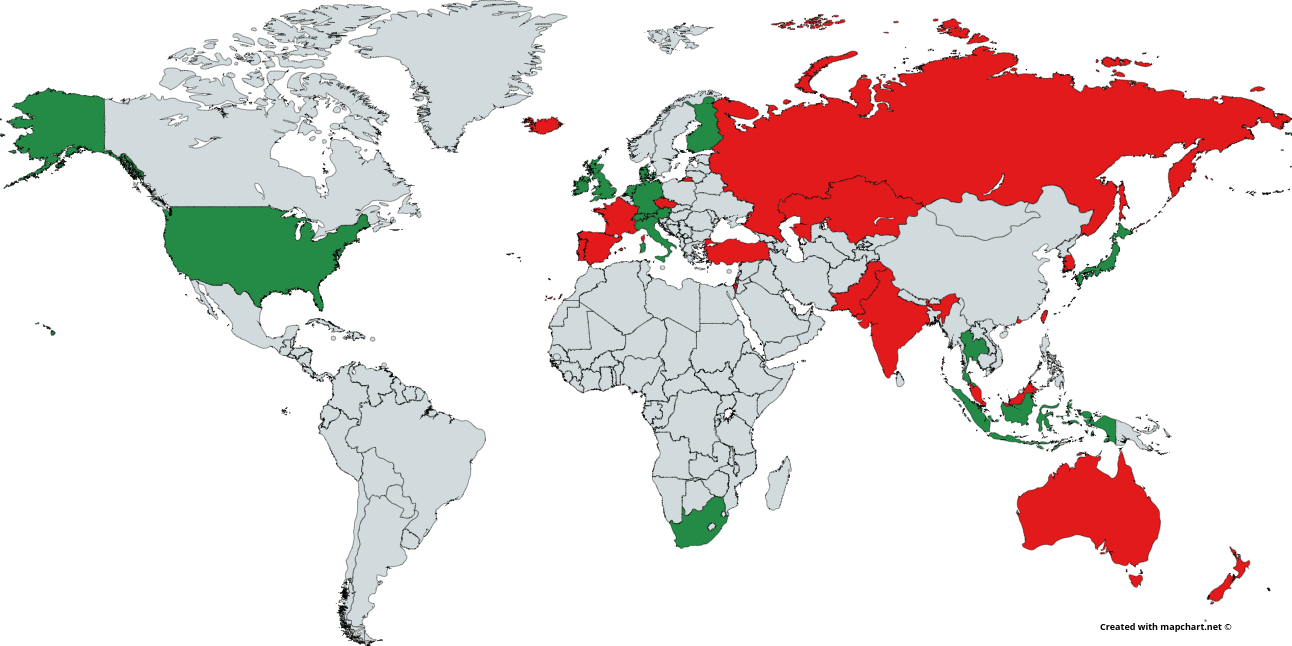
\includegraphics[scale=0.25]{figs/worldmap.png}}
    \caption{A geographical representation of countries in which \glspl{hei} were contacted. Red denotes no replies from that country, while green indicates one or more answer being submitted}
    \label{fig:worldmap}
\end{figure}

\section{Introductory questions - Question Group 1}
Table~\ref{surveyquestions} shows all questions asked in the survey according to their respective group of questions. Questions have been grouped in a manner that will present the survey results in a clear way for the reader. The first group of questions are introductory questions, concerning the respondent's current indoor mapping situation. After respondents stated their affiliation, the question "Are you currently using an indoor mapping service?" (Q1) was asked, with results shown in Figure~\ref{fig:q1}. The rationale behind this question, was to see if it was possible to churn existing \gls{ims} users to a freemium-based \gls{ims}. Conversely, respondents replying "no" are also interesting subjects for the surveyor. These represent potential first-time procurers of an \glspl{ims}, and together with those who replied "Yes" in Q2 they make up potential customers. The majority of respondents (64,1\%) had no \gls{ims} in place, while 35,9\% stated that they have an \gls{ims} in place. 

\begin{figure}[H]
    \centering
    \fbox{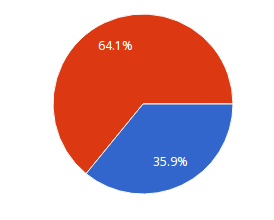
\includegraphics{figs/q1.png}}
    \caption{Q1: "Are you currently using an indoor mapping service?". Blue indicates "Yes" and red indicates "No"}
    \label{fig:q1}
\end{figure}


Based on the response given in Q1 respondents were either forwarded to Q2 or Q3. Respondents stating that they already employed an \gls{ims} were forwarded to Q3, while those without an \gls{ims} were routed to Q2. Q2 asked respondents without an \gls{ims} if they were willing to consider using an \gls{ims}. This was posed in order to gauge and measure the respondent's willingness for procurement and interest in an indoor mapping system, with results shown in Figure~\ref{fig:q2}. A total of 25 respondents replied to this question, due to this question being irrelevant for those previously stating that they already have an \gls{ims}. A majority of 68\% replied that they were willing to consider using an \gls{ims}, while 32\% stated that an indoor mapping system was not something they would consider using. To follow up on the latter group, a qualitative question in Q2.2 was asked, where respondents were asked to state the reason as to why they would not consider such a service. Question 2.2 was not mandatory, but 3 respondents chose to reply. However, these replies contributing little to the results of this thesis.


\begin{figure}[H]
    \centering
    \fbox{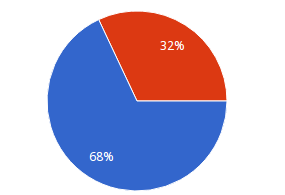
\includegraphics{figs/q2.png}}
    \caption{Q2: "Are you willing to consider using an indoor mapping service?". Blue indicates "Yes" and red indicates "No"}
    \label{fig:q2}
\end{figure}


\begin{table}[]
\centering
\caption{Questions asked in the International Market Survey}
\label{surveyquestions}
\resizebox{\textwidth}{!}{%
\begin{tabular}{|c|c|c|l|}
\hline
\textbf{Keyword} & \textbf{} & \multicolumn{1}{l|}{\textbf{\begin{tabular}[c]{@{}l@{}}Question\\ Group\end{tabular}}} & \textbf{Question phrasing}                                                                                                                                                                                                                                             \\ \hline
Q1               &           & 1                                                                                      & Are you currently using an indoor mapping service?                                                                                                                                                                                                                     \\ \hline
                 & Q2.1        & 1                                                                                      & Are you willing to consider using an indoor mapping service?                                                                                                                                                                                                           \\ \hline
                 & Q2.2      & 1                                                                                      & If no, please state the reason as to why this is not desired                                                                                                                                                                                                           \\ \hline
Q3               &           & 2                                                                                      & \begin{tabular}[c]{@{}l@{}}Given an indoor mapping service that will entail\\ several benefits for your institution, \\ please rate the initial interest in such a service\end{tabular}                                                                                \\ \hline
Q4               &           & 2                                                                                      & \begin{tabular}[c]{@{}l@{}}How much of an concern would price be in procuring \\ an indoor mapping service?\end{tabular}                                                                                                                                               \\ \hline
Q5               &           & 3                                                                                      & \begin{tabular}[c]{@{}l@{}}Please rank the following services in terms of willingness to pay: \\ "Navigation \& indoor pathfinding", "Timetable integration", \\ "Integration with SMS, apps, IT-infrastructure etc." \\ and "Automatic updating of maps"\end{tabular} \\ \hline
Q6               &           & 4                                                                                      & \begin{tabular}[c]{@{}l@{}}Which factors would be of concern when procuring\\ an indoor mapping service?\end{tabular}                                                                                                                                                  \\ \hline
\end{tabular}%
}
\end{table}

\section{Measuring Interest - Question Group 2}
This section contains questions engineered to measure the interest for \glspl{ims} in a quantitative manner. The first question Q3 was formulated as follows: "Given an indoor mapping service that will entail several benefits for your institution, please rate the initial interest in such a service". Additionally, respondents were presented with examples of how an \gls{ims} could benefit their institution~\footnote{\textit{''Improve visitor experience by showing them where to go, how to get there and even where to park. Improve employee efficiency by showing new personnel i.e. cleaning personnel around campus without the need for a dedicated guide. Improve the experience for students by alleviating stress and uncertainty by showing students and staff alike to the correct location in time for class. Additionally, an indoor mapping enables service personnel to readily locate the place of interest as opposed to decoding a textual description.''}}. Possible answers were presented on a Likert scale with 1 denoting "Not interested at all" and 5 denoting "Highly interested".


Figure~\ref{fig:q3} shows the results from Q3. Looking at the statistics from Table~\ref{q3q4stats} a mean of 3,872 and the most common answer being "Interested (4)", it can be argued that an initial interest for \glspl{ims} exists. This further reinforced by the fact that 64,1\% showed initial interest in such a service in Q1. These results can be said to conclusively point towards a definite interest in \glspl{ims} among the respondents. 32\% were initially not willing to consider using an \gls{ims} (Q2), but after being presented with the potential benefits of an \gls{ims}, this number was lowered to 15,4\%. This can be viewed as a positive trend, but it can also indicate that the market surveyed in this case is not aware of the possible positive benefits an \gls{ims} entails.


\begin{figure}
    \centering
    \fbox{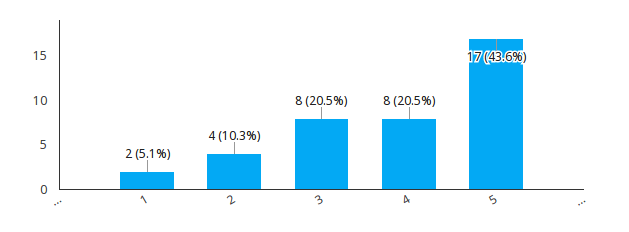
\includegraphics[width=\textwidth]{figs/q3.png}}
    \caption{Results of Q3: "Given an indoor mapping service that will entail several benefits for your institution, please rate the initial interest in such a service". Vertical axis denotes number of responses.}
    \label{fig:q3}
\end{figure}



Similar to Q3, Q4 was posed as a quantitative question and asked respondents "how much of an concern price would be in procuring an indoor mapping service". This question aimed to measure the viability of freemium in the \gls{b2bc} paradigm. A low concern for price might indicate that freemium itself is not a main proponent in accelerating customer acquisition, and conversely a high concern for price would indicate a certain viability for freemium among price-sensitive customers. Compared to Q3, this question garnered even more positive results: A mean of 4,026 and a median of 4 indicates a trend that the respondents were price-sensitive. Further cementing this notion is the fact that 76,9\% of respondents viewed price as a somewhat high to a high concern. In a non-freemium business paradigm these results would potentially be negative indicators, as price-sensitive customers could potentially lead to a elongated sales pipeline. However, in the freemium paradigm these are excellent results, since price seems to be a major factor in the potential procurement of an \gls{ims}. The results from this question can be seen in Figure~\ref{fig:q4}



\begin{table}[]
\centering
\caption{Statistics: Question Group 2}
\label{q3q4stats}
\resizebox{\textwidth}{!}{%
\begin{tabular}{|l|l|l|}
\hline
\textbf{Parameter} & \textbf{Q3: Interest} & \textbf{Q4: Concerning price} \\ \hline
Sample size        & 39                    & 39                            \\ \hline
Mean               & 3,872                 & 4,026                         \\ \hline
Median             & 4                     & 4                             \\ \hline
Mode               & Interested (4)        & Somewhat High Concern (4)     \\ \hline
\end{tabular}%
}
\end{table}


\begin{figure}
    \centering
    \fbox{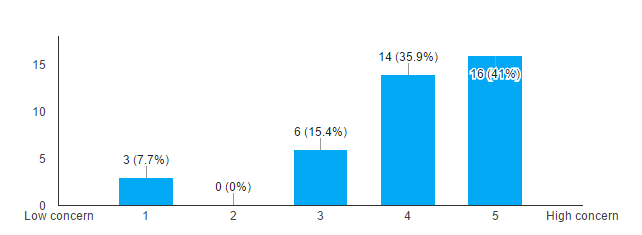
\includegraphics[width=\textwidth]{figs/q4.PNG}}
    \caption{Results of Q4: "How much of an concern would price be in procuring an indoor mapping service?" Vertical axis denotes number of responses.}
    \label{fig:q4}
\end{figure}

\section{Interest for Premium, Value-Adding Services - Group 3}
This group of questions contains one question, divided into 4 sub-questions. Thusly, the different questions will hereby be referred to as Q5.1, Q5.2, Q5.3 and Q5.4. For this group of questions, respondents were asked to rank four different \gls{ims}-related services in terms of willingness to pay, where 1 indicated a low willingness to pay, and 5 indicating a high willingness to pay. Under each service, the respondents were informed about why these features might be beneficial to their institution, akin to Q3. The statistics of these questions can be seen in Table~\ref{q5stats}. In the freemium paradigm with the few paying for the many, it is important that premium features are implemented for the sake of profitability. However, freemium in a \gls{b2b} or \gls{b2bc} market is more than often used as a potent leads-generator~\cite{jepson2009freemium}. Due to this, the willingness to pay for the premium features are not detrimental for successfully applying freemium in this case, thus making any negative feedback on premium, value-adding services not necessarily speak against freemium. Lastly, it should be noted that any initial disinterest from respondents are further compounded in this group of questions, and the numbers should be viewed accordingly.

\begin{table}[]
\centering
\caption{Statistics: Question Group 3}
\label{q5stats}
\resizebox{\textwidth}{!}{%
\begin{tabular}{|l|l|l|l|l|}
\hline
\textbf{Parameter}      & \textbf{Q5.1} & \textbf{Q5.2} & \textbf{Q5.3} & \textbf{Q5.4} \\ \hline
Sample size             & 39            & 39            & 39            & 39            \\ \hline
Mean                    & 2.59          & 2.538         & 2.769         & 2.872         \\ \hline
Median                  & 3             & 3             & 3             & 3             \\ \hline
Mode                    & Neutral (3)   & Neutral (3)   & Neutral (3)   & Neutral (3)   \\ \hline
Willing to pay (4 \& 5) & 24.4\%        & 31,7\%        & 31,7\%        & 36.6\%        \\ \hline
\end{tabular}%
}
\end{table}


For this Q5.1 the respondents were given the following potentially beneficial features of indoor navigation and pathfinding:

\begin{displayquote}
\textit{''While not a necessary component of an indoor mapping service, navigation and indoor path finding can help users find their desired location. A plethora of technologies exist for this purpose using existing Wi-Fi infrastructure, Bluetooth, beacons, smartphone sensors, magnetic positioning etc.''}
\end{displayquote}

Figure~\ref{fig:q51} shows results from Q5.1. The statistics show a mean of 2,59 and a median of 3 making the mode "Neutral (3)". These numbers do not indicate a strong willingness or lack thereof of this particular feature, and represents the third most popular premium service. The numbers are however, slightly on the positive side of the scale with a non-negative median, however there were equally many neutral as there were those with low willingness to pay for this type of service. \gls{mm} has stated that their primary focus is making the indoor maps themselves, and as much as 80\% of its users do not use any form of indoor navigation (Jelle, personal communication 17.09.2015). This fact is to some extent reflected in these results. The respondents were however not informed that an \gls{ims} such as \gls{mm} has a partner in Cisco that enables the usage of existing Wi-Fi infrastructure for positioning and navigation. Given that indoor navigation techniques are in its infancy, it can perhaps be expected to see a rise in the technologies applied in this field in the future. 

\begin{figure}[H]
    \centering
    \fbox{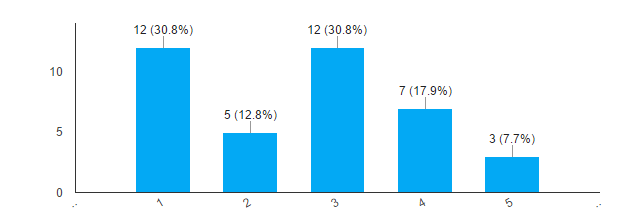
\includegraphics[width=\textwidth]{figs/q51.PNG}}
    \caption{Results of Q5.1: "Navigation and indoor pathfinding". Vertical axis denotes number of responses.}
    \label{fig:q51}
\end{figure}

Q5.2 asked the users to rate their willingness to pay for timetable integration. Respondents were presented with the following potential benefits:

\begin{displayquote}
\textit{'' "Where", "how" and "when" are commonly asked questions when an appointment is due or a meeting is taking place. Timetable integration aims to answer the two former questions by providing an indoor map and which path to take to get there.''}
\end{displayquote}

With a mean of 2,538 and a median of 3, this was the least popular of the presented value-adding services. Figure~\ref{fig:q52} shows the results being quite even on all but one of the possible answers, likely indicating a divided set of responders. As with Q5.1, these numbers to not indicate any trends of strong or weak desires towards this type of service, but it is important to emphasise that some respondents were unfamiliar with \glspl{ims} in general, or had no desire to acquire one. In hindsight, the author could have provided respondents of the survey with visual rather than textual examples of the value-adding, premium services to give respondents a better overview of the implications and usefulness of these services. 


\begin{figure}[H]
    \centering
    \fbox{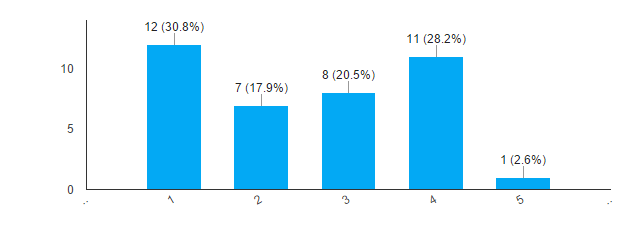
\includegraphics[width=\textwidth]{figs/q52.PNG}}
    \caption{Results of Q5.2: "Timetable integration". Vertical axis denotes number of responses.}
    \label{fig:q52}
\end{figure}


The next question in the group concerned the integration of an \gls{ims} into SMS, applications, IT-infrastructure etc. Potential benefits were proclaimed as follows:

\begin{displayquote}
\textit{"An API that integrates indoor maps with the existing services mentioned above, aims to enable seamlessly integrating indoor maps into already existing systems and services without the need to manually do so for every service."}
\end{displayquote}

The results of this question can be seen in Figure~\ref{fig:q53}, with a mean of 2.769 and median of 3 making it the second most popular service presented, with 61,6\% of replies being Neutral (3) and above. As stated previously, it must be stressed that it might be hard to visualise how these premium features work in a concrete scenario. If potential \gls{ims} buyers are largely unaware of the benefits, it can make this particular service a hard sell. Furthermore, integrating an \gls{ims} into existing infrastructure might represent a security risk for the procuring part. This pertains to any potential security holes an \gls{ims} might have, and if such holes are present, malicious users are potentially able to gather sensitive data such as passwords and user-names. Therefore, it was expected that this question would score low, but the results shows it being on par with the others.  

\begin{figure}[H]
    \centering
    \fbox{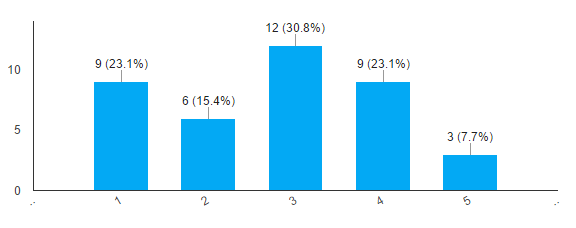
\includegraphics[width=\textwidth]{figs/q53.PNG}}
    \caption{Results of Q5.3: "Integration with SMS, apps, IT-infrastructure etc.
". Vertical axis denotes number of responses.}
    \label{fig:q53}
\end{figure}

The last question in the group, Q5.4, asked respondents to rate a service that automatically kept maps up to date. Respondents were presented with the following key features of this particular value-adding service:

\begin{displayquote}
\textit{''Larger establishments tend to change over time, and often see around 10\% of buildings change annually\footnote{Jelle, personal communication, 25.09.2015}. Manually updating indoor maps can therefore be a tedious and time-consuming activity.''}
\end{displayquote}

Figure~\ref{fig:q54} shows results from Q5.4, with a mean of 2.872 and a median of 3 (Neutral). For respondents unaccustomed to \glspl{ims}, this question would perhaps be the hardest to answer, since it directly revolves around an \gls{ims}. As stated in earlier, \glspl{hei} may see over 10\% of its structures change during the course of a year. This is possibly reflected in the statistics, as they show this feature being the most popular of the four. It also had the highest number of interested respondents at 35,9\%. It can be speculated that the \glspl{hei} contacted in relation to the survey were aware that updating floor-plans could be quite an undertaking, and an \gls{ims} with this feature would be well received. 


\begin{figure}[H]
    \centering
    \fbox{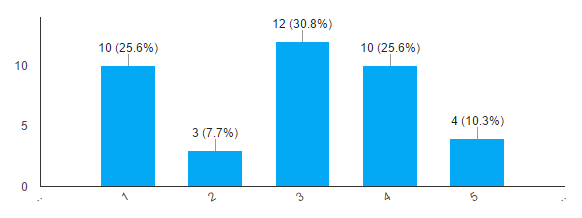
\includegraphics[width=\textwidth]{figs/q54.PNG}}
    \caption{Results of Q5.4: "Automatic updating of maps". Vertical axis denotes number of responses.}
    \label{fig:q54}
\end{figure}

\newpage

\section{Potential Procurement Concerns - Question Group 4}
The final group of questions asked concerned potential aversions that the \glspl{hei} contacted might have. At the end of the survey, respondents were welcome to freely add anything concerning the survey, the free model or \glspl{ims}, but few chose to do this. The rationale behind having this question group was to map the potential hindrances in procurement of an \gls{ims}. The question asked in this section consisted of checkboxes where respondents were free to mark as many options as desired, and an overview of the replies is shown in Table~\ref{q6}. Respondents were free to interpret "Security Concerns" in their own way. However, it was the author's intention to gauge if the respondent owning the rights to the indoor maps themselves was a concern or not.


\begin{table}[H]
\centering
\caption{Overview of data from Q6}
\label{q6}
\begin{tabular}{l|l|l|l|l|}
\cline{2-5}
                                           & \textbf{Price} & \textbf{Demand} & \textbf{Security Concerns} & \textbf{Other} \\ \hline
\multicolumn{1}{|l|}{\textbf{Sample size}} & 39             & 39              & 39                         & 39             \\ \hline
\multicolumn{1}{|l|}{\textbf{Quantity}}    & 33             & 19              & 23                         & 8              \\ \hline
\multicolumn{1}{|l|}{\textbf{Percentage}}  & 84.6\%         & 48.7\%          & 59.0\%                     & 20.5\%         \\ \hline
\end{tabular}
\end{table}

Q6, the final question of the survey prompted the respondents with the following: "Which factors would be of concern when procuring an indoor mapping service?" Four different factors were presented, and respondents were allowed to choose all four should they so desire, with the different options being "Price", "Demand", "Security concerns" and "Other". The "Other"-option allowed respondents to shortly describe a potential concern not applicable to the above. The results of this question can be seen in Figure~\ref{fig:q6}, and some of the "other"-factors were suggested as follows:
\begin{itemize}
    \item \textit{''Accuracy and legibility''}
    \item \textit{''Maintenance''}
    \item \textit{''Integration with reservation system''}
    \item \textit{''Ease of use, accessibility and [the] ability to administer system locally''}
    \item \textit{''Quality of the service such as usability and features''}
    \item \textit{''Content''}
    \item \textit{''Campus user experience''}
\end{itemize}
\newpage
Some of these factors pertains to the actual usefulness of the service itself, while some concern the user experience. Although \gls{b2b} and \gls{b2bc} markets have many similarities, this can be said to be a difference in this case: As the purchasing business in a \gls{b2bc} scenario governs the the service provided to its clients, quality, ease of use and usefulness are factors that must not be overlooked in the case for \glspl{hei}.



\begin{figure}[H]
    \centering
    \fbox{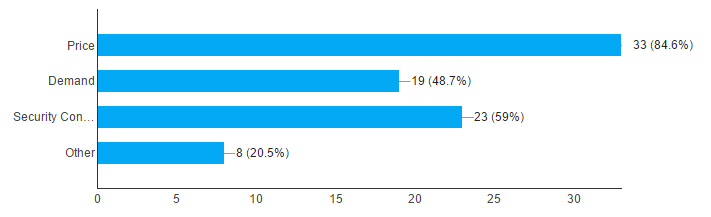
\includegraphics[width=\textwidth]{figs/q6.PNG}}
    \caption{Results of Q6: "Which factors would be of concern when procuring an indoor mapping service?". Horizontal axis represents number of responses. Option 3 not wholly visible: "Security Concerns".}
    \label{fig:q6}
\end{figure}

The most chosen factor was "Price" at 84,6\%, followed by "Security Concerns" at 59\%, "Demand" at 48,7\% and "Other" at 20,5\%. Given that Q4 showed that most of the respondents were concerned about price, this trend is further confirmed in this question. For unaware readers, it might be hard to grasp that citing "Price" is not a given factor in the procurement of a service or product. It is interesting however, due to the market segment discussed in this thesis (\glspl{hei}) might not be as price sensitive as other parts of the market. Many of these are publicly owned, and as such long-running costs may be more of a concern. In the case of potential public procurements, countries in the EU and countries like Norway have laws regarding public procurement practises and regulation~\cite{europeancommision}\cite{procurement}. In the preliminary research paper, the author reviewed a similar research question constrained to the Norwegian market. In terms of Norway's public procurement laws, it is stated that if any public entity wishes to purchase a certain service, that type of service has to be announced publicly. Offering-bids from outreachers is usually the norm, and after a certain amount of time, an eventual procurement can take place. A similar survey was offered in this paper where one respondent from a Norwegian Hospital stated~\cite{kristiantagesen2015}:
\newpage
\begin{displayquote}
\textit{''We have to deal with the rulings of public procurement, and it would be the total cost that is the underlying factor. The content of the "basic" package is detrimental to a potential procurement, as it may trigger further needs for more services. If a(n) [indoor mapping] system can satisfy the demands and rules of a public procurement, then [a freemium-based \gls{ims}] is of interest''.}
\end{displayquote}
In terms of the viability of freemium in this scenario, this can be viewed positively and negatively: The positive aspect of this is that potential leads and prospects in an organisation that is in a procurement phase, might convince senior management personnel more easily, to obtain a service that will cost nothing initially. On the other hand, long-term and total costs may be more concerning for potential procurers than a service or product being free initially. As stated by the above respondent, the contents of the non-premium parts were detrimental, and may trigger the need for purchasing premium parts of the product or service.